 \documentclass[a4paper, 12pt,twoside]{book}

% set the paper size and the margins
\usepackage[top = 2cm, bottom = 2cm, left = 2cm, right = 4cm ]{geometry}
\usepackage[showboxes]{textpos}
\setlength{\TPHorizModule}{10mm}
\setlength{\TPVertModule}{\TPHorizModule}
\TPMargin{2mm}
% set the header and the footnote
\usepackage{fancyhdr}
% Supress the hyphenation
\hyphenation{thatshouldnot} 
% for table and equations
\usepackage{tablefootnote}
\usepackage{amsmath,amsfonts,amsthm}
\usepackage{multirow}
\usepackage{hhline}
% make a wide hat for the least-squares regression line
 \usepackage{scalerel,stackengine}
\stackMath
\newcommand\reallywidehat[1]{%
\savestack{\tmpbox}{\stretchto{%
  \scaleto{%
    \scalerel*[\widthof{\ensuremath{#1}}]{\kern-.6pt\bigwedge\kern-.6pt}%
    {\rule[-\textheight/2]{1ex}{\textheight}}%WIDTH-LIMITED BIG WEDGE
  }{\textheight}% 
}{0.5ex}}%
\stackon[1pt]{#1}{\tmpbox}%
}
\usepackage[shortlabels]{enumitem}

% knitr packages
\usepackage[]{graphicx}
\usepackage[]{color}
%% maxwidth is the original width if it is less than linewidth
%% otherwise use linewidth (to make sure the graphics do not exceed the margin)
\makeatletter
\def\maxwidth{ %
  \ifdim\Gin@nat@width>\linewidth
    \linewidth
  \else
    \Gin@nat@width
  \fi
}
\makeatother

\definecolor{fgcolor}{rgb}{0.345, 0.345, 0.345}
\newcommand{\hlnum}[1]{\textcolor[rgb]{0.686,0.059,0.569}{#1}}%
\newcommand{\hlstr}[1]{\textcolor[rgb]{0.192,0.494,0.8}{#1}}%
\newcommand{\hlcom}[1]{\textcolor[rgb]{0.678,0.584,0.686}{\textit{#1}}}%
\newcommand{\hlopt}[1]{\textcolor[rgb]{0,0,0}{#1}}%
\newcommand{\hlstd}[1]{\textcolor[rgb]{0.345,0.345,0.345}{#1}}%
\newcommand{\hlkwa}[1]{\textcolor[rgb]{0.161,0.373,0.58}{\textbf{#1}}}%
\newcommand{\hlkwb}[1]{\textcolor[rgb]{0.69,0.353,0.396}{#1}}%
\newcommand{\hlkwc}[1]{\textcolor[rgb]{0.333,0.667,0.333}{#1}}%
\newcommand{\hlkwd}[1]{\textcolor[rgb]{0.737,0.353,0.396}{\textbf{#1}}}%
\let\hlipl\hlkwb
\usepackage{framed}
\makeatletter
\newenvironment{kframe}{%
 \def\at@end@of@kframe{}%
 \ifinner\ifhmode%
  \def\at@end@of@kframe{\end{minipage}}%
  \begin{minipage}{\columnwidth}%
 \fi\fi%
 \def\FrameCommand##1{\hskip\@totalleftmargin \hskip-\fboxsep
 \colorbox{shadecolor}{##1}\hskip-\fboxsep
     % There is no \\@totalrightmargin, so:
     \hskip-\linewidth \hskip-\@totalleftmargin \hskip\columnwidth}%
 \MakeFramed {\advance\hsize-\width
   \@totalleftmargin\z@ \linewidth\hsize
   \@setminipage}}%
 {\par\unskip\endMakeFramed%
 \at@end@of@kframe}
\makeatother


\definecolor{shadecolor}{rgb}{.97, .97, .97}
\definecolor{messagecolor}{rgb}{0, 0, 0}
\definecolor{warningcolor}{rgb}{1, 0, 1}
\definecolor{errorcolor}{rgb}{1, 0, 0}
\newenvironment{knitrout}{}{} % an empty environment to be redefined in TeX

\usepackage{alltt}


% packages will be used by the 'kable' package
\usepackage{booktabs}
\usepackage{longtable}
\usepackage{array}
\usepackage{multirow}
\usepackage[table]{xcolor}
\usepackage{wrapfig}
\usepackage{float}
\usepackage{colortbl} 
\usepackage{pdflscape}
\usepackage{tabu}
\usepackage{threeparttable}
\usepackage{threeparttablex}
\usepackage[normalem]{ulem}
\usepackage{makecell}
\usepackage{xcolor}
\IfFileExists{upquote.sty}{\usepackage{upquote}}{}

% define a color for highlight
\definecolor{asparagus}{rgb}{0.53, 0.66, 0.42}
\definecolor{babypink}{rgb}{0.96, 0.76, 0.76}
\definecolor{champagne}{rgb}{0.97, 0.91, 0.81}
\definecolor{forestgreen}{rgb}{0.13, 0.55, 0.13}
\definecolor{dollarbill}{rgb}{0.52, 0.73, 0.4}

\usepackage{tcolorbox}

\tcbset{width=0.9\textwidth,boxrule=0pt,colback=champagne,arc=0pt,
auto outer arc,left=0pt,right=0p}

\usepackage{hhline}

\usepackage{amsmath}

\setlength{\parindent}{0.5cm} 

\usepackage{siunitx}

%Chinese yen
\usepackage{stackengine}
\newcommand{\textyen}{\stackengine{-6pt}{=}{\large{\text{Y}}}{O}{c}{F}{T}{S}}

\setlength{\parindent}{0cm}

\begin{document}

%Deal with the headers of each chapter
\pagestyle{fancy}
\fancyhf{}
\renewcommand{\chaptermark}[1]{ \markboth{#1}{} }
\fancyhead[CE,CO]{\leftmark}
\fancyfoot[LE,RO]{\thepage}
\chapter{Inference for Distributions of Categorical Data}

Is a hypothesized distribution valid for a categorical variable? Whether the distribution of a categorical variable differs for two or more populations or treatments? Is there an association between two categorical variables in a population? We will solve those three types of problems in this chapter by performing $\chi^2$ tests.
\newpage

\section{Chi-square test for goodness of fit}
\textbf{Take a look at the following problem.}\vspace{0.3cm}

 According to the Census Bureau, the 
 distribution by ethnic background of the New York City population in a recent year was \vspace{0.3cm}
 
 Hispanic: 28\% \hspace{0.2cm} Black: 24\%\hspace{0.2cm} White: 35\% \hspace{0.2cm}Asian: 12\% \hspace{0.2cm}Others: 1\%\vspace{0.3cm}
 
The manager of a large housing complex in the city wonders whether the distribution by race of the complex's residents is consistent with the population distribution. To find out, she records data from a random sample of 800 residents. The table below displays the sample data.
    \begin{table}[H]
    \centering
    \begin{tabular}{lcccc c}
    \hline
   \textbf{Race:}& \textbf{Hispanic}& \textbf{Black}& \textbf{White} &\textbf{Asian} &\textbf{Other}\\
   \textbf{Count:}& 212 &202 &270 &94 &22\\
   \hline
    \end{tabular}
    \caption{Observed residents of different races}
    \label{Observed}
    \end{table}     
Are these data significantly different from the city’s distribution by race? Carry out an appropriate test at the $\alpha = 0.05$ level to support your answer. 

\begin{itemize}
   \item \textbf{The test statistic $\chi^2$}\vspace{0.3cm}

  The hypotheses for the above problem can be set as\vspace{0.3cm}
  
  $\textbf{H}_0:$ The race distribution in the complex is the same as in the New York City.\\
   $\textbf{H}_a:$ The race distribution in the complex different from in the New York City.\vspace{0.3cm}

As the hypotheses tests we learned before, we need to calculate a P-value and compare it with the significance level $\alpha$. Let's recall the definition of P-value.\vspace{0.3cm}

\colorbox{babypink}{\parbox{0.9\textwidth}{
\textbf{P-value} is the probability, computed assuming $H_0$ is true, that the statistic(such as $\bar{x}$ and $\reallywidehat{p}$) would be as extreme as or more extreme than the observed value, in the direction of $H_a$.
}}
\vspace{0.3cm}

Therefore, we have to find a  statistic before we calculate the P-value. This statistic is $\chi^2$.
$$\chi^2 = \sum\frac{(\text{Observed}- \text{Expected})^2}{\text{Expected}}$$

$\chi^2$ is also a \textit{test statistic}, because it plays the same role as the \textit{test statistic $z$} or \textit{test statistic $t$} in calculating the P-value.\vspace{0.3cm}

The ``Observed'' in the formula means the observed value. Table \ref{Observed} gives the observed values.\vspace{0.3cm}

The ``Expected'' in the formula means the expected value if $\textbf{H}_0$ is true. In the above problem, the ``Expected'' are given below. 
    \begin{table}[H]
    \scalebox{0.8}{
    \begin{tabular}{lcccc c}    
    \hline
   \textbf{Race:}& \textbf{Hispanic}& \textbf{Black}& \textbf{White} &\textbf{Asian} &\textbf{Other}\\
   \textbf{Expected:}&$800\times 28\% = 224$ &$800\times 24\% = 192$&$800\times 35\% = 280$ &$800\times 12\% = 96$ &$800\times 1\% = 8$\\
   \hline   
    \end{tabular}}
    \caption{Expected number of residents of different races}
    \label{Expected}
    \end{table} 

Now let's plug in the values and calculate $\chi^2$
$$\chi^2 = \frac{(212-224)^2}{224}+\frac{(202-192)^2}{192}+
\frac{(270-280)^2}{280}+\frac{(94-96)^2}{96}+\frac{(22-8)^2}{8}= 26.1$$

\begin{textblock}{3}(15.5, -2)
\textblockcolor{dollarbill}
Is a larger $\chi^2$ or a smaller $\chi^2$ in favour of $\textbf{H}_a$?
\end{textblock}
\item \textbf{$\chi^2$ distribution}\vspace{0.3cm}

We have to know the sampling distribution of $\chi^2$ in order to calculate the P-value. $\chi^2$ follows a $\chi^2$ distribution with \textit{degree of freedom $df=n-1$}. $n$ is the number of categories.  In the above example, $n = 5$, $df = 5-1=4$. 
    \begin{figure}[H]
    \centering
    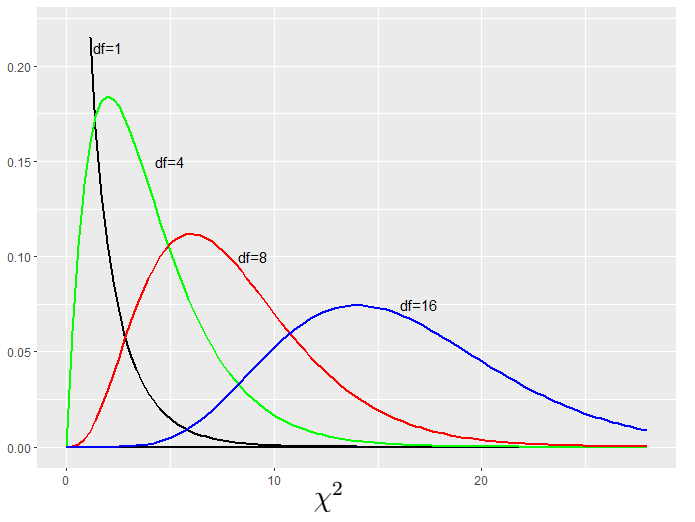
\includegraphics[scale=0.6]{Chi-squareDistribution}
    \caption{$\chi^2$ distribution with different degree of freedom}
    \label{Chi-squareDistribution}
    \end{figure}
From figure \ref{Chi-squareDistribution}, we can see that the sampling distribution of $\chi^2$ becomes more and more symmetric as the degree of freedom increase.

\item \textbf{P-value}\vspace{0.3cm}

According to the definition of the P-value, it should be the probability of $\chi^2$ larger than the observed value of $\chi^2$
$$\textbf{P-value}=\textbf{P}(\chi^2 > 26.1) = 0.0003 \qquad df = 5-1 =4$$
Clearly the P-value is smaller than the given significance level $\alpha = 0.05$. We reject $\textbf{H}_0$, and have convincing evidence that the distribution of races in this complex is difference from that in the New York city.\vspace{0.3cm}

\item \textbf{Follow-up analysis}\vspace{0.3cm}

If the sample data lead to a statistically significant result, we can conclude that there is convincing evidence that the distribution of the categorical variable is different from the stated one.  By analysing the \textbf{components} of the $\chi^2$, we can find out which one contributes the most. \vspace{0.3cm}

In the above example, the \textit{components} of $\chi^2$ are
$$\frac{(212-224)^2}{224},\;\frac{(202-192)^2}{192},\;
\frac{(270-280)^2}{280},\;\frac{(94-96)^2}{96},\;\frac{(22-8)^2}{8} $$

$\frac{(22-8)^2}{8} = 24.5$ contributes the most to $\chi^2 = 26.1$. The proportion of ``other'' ethnic groups is larger in this complex than in that in the New York city.
\end{itemize}

\newpage

\textbf{The general steps for the \textit{Chi-square test for goodness of fit} is the same as all the other tests we learned before.}\vspace{0.3cm}

\colorbox{champagne}{\parbox{\textwidth}{
\textbf{Mendelian inheritance }\vspace{0.3cm}

Biologists wish to mate pairs of fruit flies having genetic makeup RrCc, indicating that each has one dominant gene (R) and one recessive gene (r) for eye color, along with one dominant (C) and one recessive (c) gene for wing type. Each offspring will receive one gene for each of the two traits from each parent. The following table, known as a Punnett square, shows the possible combinations of genes received by the offspring:
    \begin{table}[H]
    \centering
       \begin{tabular}{ccccc}
       \hline
       &\multicolumn{4}{c}{\textbf{Parent 2 passes on:}}\\
       \textbf{Parent 1 passes on:}&\textbf{RC} &\textbf{Rc} &\textbf{rC} &\textbf{rc}\\
       \textbf{RC} &RRCC(x)&RRCc(x)&RrCC(x)&RrCc(x)\\
       \textbf{Rc}& RRCc(x)&RRcc(y)&RrCc(x)&Rrcc(y)\\
       \textbf{rC}&RrCC(x)&RrCc(x)&rrCC(z)&rrCc(z)\\
       \textbf{rc}&RrCc(x)&Rrcc(y)&rrCc(z)&rrcc(w)\\
       \hline
       \end{tabular}
    \end{table}
    
    Any offspring receiving an R gene will have red eyes, and any offspring receiving a C gene will have straight wings. So based on this Punnett square, the biologists predict a ratio of 9 red-eyed, straight-winged (x); 3 red-eyed, curly-winged (y); 3 white-eyed, straightwinged (z); 1 white-eyed, curly-winged (w) offspring.\vspace{0.3cm}
    
    To test their hypothesis about the distribution of offspring, the biologists mate a random sample of pairs of fruit flies. Of 200 offspring, 99 had red eyes and straight wings, 42 had red eyes and curly wings, 49 had white eyes and straight wings, and 10 had white eyes and curly wings. Do these data differ significantly from what the biologists have predicted? Carry out a test at the $\alpha = 0.01$ significance level.
}}
\newpage

\section{Inference for two-way tables}






















\end{document}